\documentclass[a4paper]{scrartcl}
\usepackage[cm]{fullpage}
\usepackage{tabulary}
\usepackage{graphicx, caption, subcaption}

\begin{document}

\title{Sorting Algorithm Identification with Algorithmic Complexity Analysis}
\author{Donny Yang and Sean Yeoh}
\date{2015-09-02}
\maketitle

\section{Introduction}
An attempt to identify the used sorting algorithm of the given two programs using sorting algorithms from a specified limited pool of potential methods through observing its time, space and stability data. By extrapolating from the limited description of the algorithms within the pool, and usage of specific tests, it is possible to identify which were used for each program.

\section{Materials and Methods}
\begin{table}
    \centering
    \begin{tabulary}{\linewidth}{c | C | C | C | C | C | C | C}
        & Bubble & Insertion & Selection & Merge & Unstable Quick & Shell & Bogo \\
        \hline
        Best Case Time & \(O(n^2)\) or \(O(n)\)* & \(O(n)\) & \(O(n^2)\) & \(O(n \log{n})\) &  \(O(n \log{n})\) &  \(O(n \log{n})\) & \(O(1)\) \\
        Worst Case Time & \(O(n^2)\) & \(O(n^2)\) & \(O(n^2)\) & \(O(n \log{n})\) & \(O(n^2)\) & \(O(n^2)\) & \(O(\infty)\) \\
        Average Case Time & \(O(n^2)\) & \(O(n^2)\) & \(O(n^2)\) & \(O(n \log{n})\) & \(O(n \log{n})\) & ** & \(O(n!)\) \\
        Auxillary Space & \(O(1)\) & \(O(1)\) & \(O(1)\) & \(O(n)\) & \(O(\log{n})\) & \(O(1)\) & \(O(1)\) \\
        Stable? & Either* & Yes & Yes & Yes & No & No & No \\
        Pure? & Yes & Yes & Yes & Yes & Either* & Yes & No
    \end{tabulary}
    \caption{General complexity and stability of classes of algorithms \\ **: Depends on implementation \\ ***: Unknown, but thought to be around \(O(n^\frac43)\) or \(O(n^\frac54)\)}
    \label{tab:complexity}
\end{table}

\begin{table}
    \centering
    \begin{tabulary}{\linewidth}{c | C | C}
        Type & ``Oblivious'' & ``Early Exit'' \\
        \hline
        Description & Unstable and unoptimised bubble sort & Stable bubble sort that terminates when there have been no exchanges in one pass \\
        \hline
        Distinction & Results in \(O(n^2)\) best case time complexity & Results in \(O(n)\) best case time complexity
    \end{tabulary}
    \caption{Variations of Bubble Sorts}
    \label{tab:bubble_sorts}
\end{table}

\begin{table}
    \centering
    \begin{tabulary}{\linewidth}{c | C | C}
        Type & ``Vanilla'' & ``Binary Search'' \\
        \hline
        Description & Insert by swapping with previous until location is found & Binary search for location and then swap the element down to the location \\
        \hline
        Distinction & Effectively none & Effectively none
    \end{tabulary}
    \caption{Variations of Insertion Sorts}
    \label{tab:insertion_sorts}
\end{table}

\begin{table}
    \centering
    \begin{tabulary}{\linewidth}{c | C | C}
        Type & ``Vanilla'' & ``Quadratic'' \\
        \hline
        Description & Sort entire list immediately & First selection sort groups of size \(\sqrt{n}\) \\
        \hline
        Distinction & Time complexity is \(O(n^2)\) & Time complexity is \(O(n^\frac32)\).
    \end{tabulary}
    \caption{Variations of Selection Sorts}
    \label{tab:selection_sorts}
\end{table}

\begin{table}
    \centering
    \begin{tabulary}{\linewidth}{c | C | C | C}
        Type & ``Vanilla'' & ``Median of Three'' & ``Randomised'' \\
        \hline
        Description & Pivot is last element & Pivot is the median of first last and middle elements & List is shuffled then vanilla quick-sorted \\
        \hline
        Distinction & ``Pure'', but \(O(n^2)\) on already sorted lists & Avoid shitty \(O(n^2)\) worst cases. Is ``pure'' (i.e. same results for same set of data) & Also avoids shitty \(O(n^2)\) worst cases. Is ``impure''.
    \end{tabulary}
    \caption{Variations of Unstable Quick Sorts}
    \label{tab:quick_sorts}
\end{table}

\begin{table}
    \centering
    \begin{tabulary}{\linewidth}{c | C | C}
        Type & ``\(4^n\)'' & ``Modified Sedgewick'' \\
        \hline
        Description & Intervals: ..., 4096, 1024, 256, 64, 16, 4, 1 & Intervals: ..., 4193, 1073, 281, 23, 8, 1 \\
        \hline
        Distinction & Worst case: \(O(n^2)\) & Worst Case: \(O(n^{\frac{4}{3}})\)
    \end{tabulary}
    \caption{Variations of Shell Sorts}
    \label{tab:shell_sort}
\end{table}

The pool of data provided contained 13 algorithms, composed of variations upon 7 basic sorts. Of these 7 basic sorts, general characteristics for time and space complexity and sorting stability can be distinguished to classify each `class' of sorting algorithm (Table \ref{tab:complexity}) by comparing the best case (already sorted data), worst case (reverse sorted data), average case (randomized data) timing data, stability of results and memory usage size.

Given the general matrix provided in Table \ref{tab:complexity}, it is easy to deduces which `class' of algorithm the sort is using if given the results for best/worst/average case time complexities, space complexity, stability and purity. Through analysing the results, we can accurately deduce which of the 7 `classes' the sort belongs to given the 5 indicators, except between ``Early Exit'' Bubble sort and Insertion sort.

Data was collected from GNU \texttt{time}, using its user time and maximum resident set size.

By applying tests of a non-degenerate time duration, producing size--time and size--space pairs, the data was fitted to various expected functions, and the most reasonable fit was chosen as the resulting complexity.

Additionally, `Fixed case' would have been tested if needed to distinguish between certain algorithms, but this did not turn out to be required.

\subsection{Special Case for Sort A}
A partially ordered and partially reversed set of data is necessary to distinguish between Early Exit Bubble Sort and Insertion Sort given they have identical Best/Worst/Average time and space complexities. The first \(n - k\) elements are ordered and the last \(k\) elements are in reverse order. Notably, Bubble sort would exhibit \(O(n k)\), whereas Insertion sort would exhibit \(O(k^2)\) complexity on the same set of data.

\subsection{Special Case for Sort B}
A `riffle sorted' set of data is necessary to distinguish between \(4^n\) and Sedgewick Shell Sort and Median-Of-Three Quick Sort given they have indistinguishable Best/Worst/Average time complexities and effectively indistinguishable time complexities.
`Riffle sorting' is where elements greater and smaller than the median occupy odd and even positions, as if a new deck of cards were `riffle shuffled' as outlined by the infinitely reliable Wikipedia. Notably, \(4^n\) Shell Sort would exhibit \(O(n^2)\) complexity on this custom data set, whereas Median-Of-Three Quick Sort would maintain \(O(n \log{n})\) and Sedgewick Shell Sorting would yield an average case time less than \(O(n^\frac43)\).


\section{Results}
\begin{figure}[p]
    \centering
    \begin{subfigure}[b]{0.45\textwidth}
        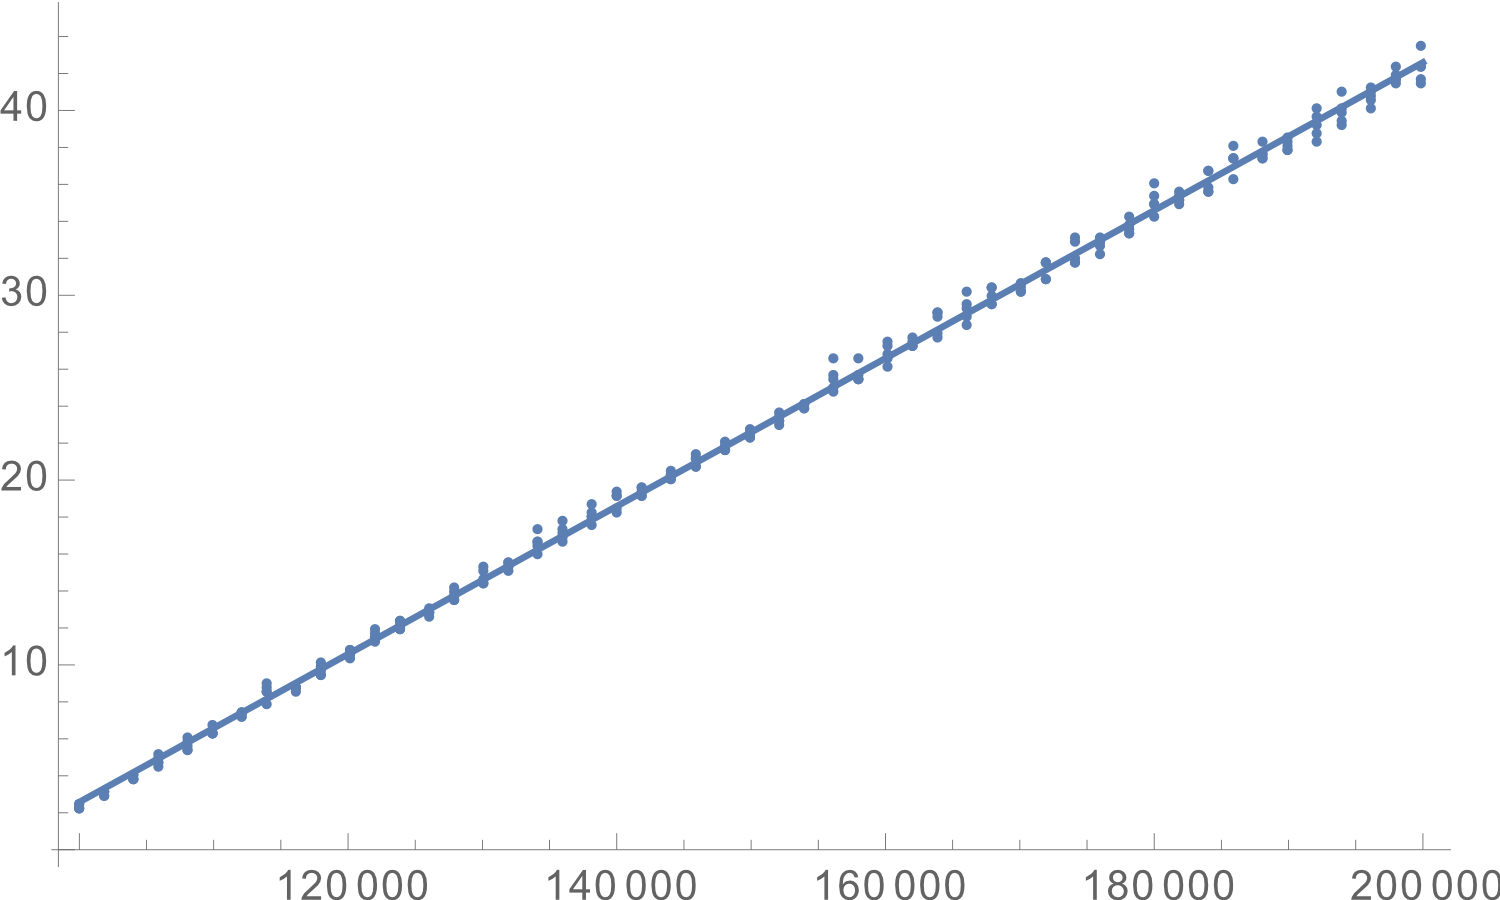
\includegraphics[width = \textwidth]{sortA_ordered_time.png}
        \caption{Time: \((5.7 \times 10^{-7}) n - 0.0019\)}
    \end{subfigure}
    ~
    \begin{subfigure}[b]{0.45\textwidth}
        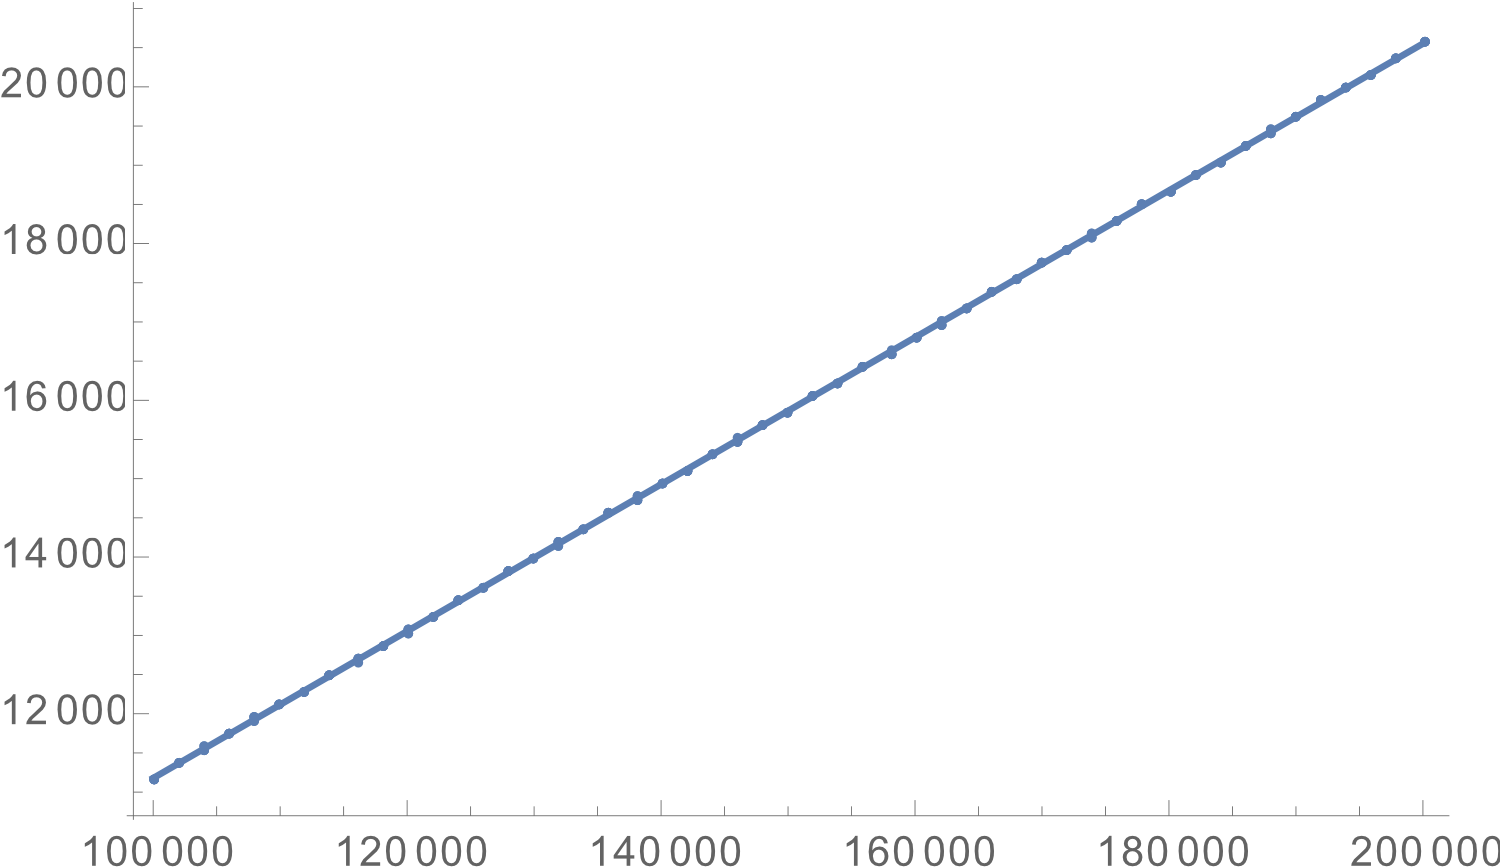
\includegraphics[width = \textwidth]{sortA_ordered_space.png}
        \caption{Space: \(0.094 n + 1800\)}
    \end{subfigure}
    \caption{Sort A - Ordered}
    \label{fig:sortA_ordered}
\end{figure}

\begin{figure}[p]
    \centering
    \begin{subfigure}[b]{0.45\textwidth}
        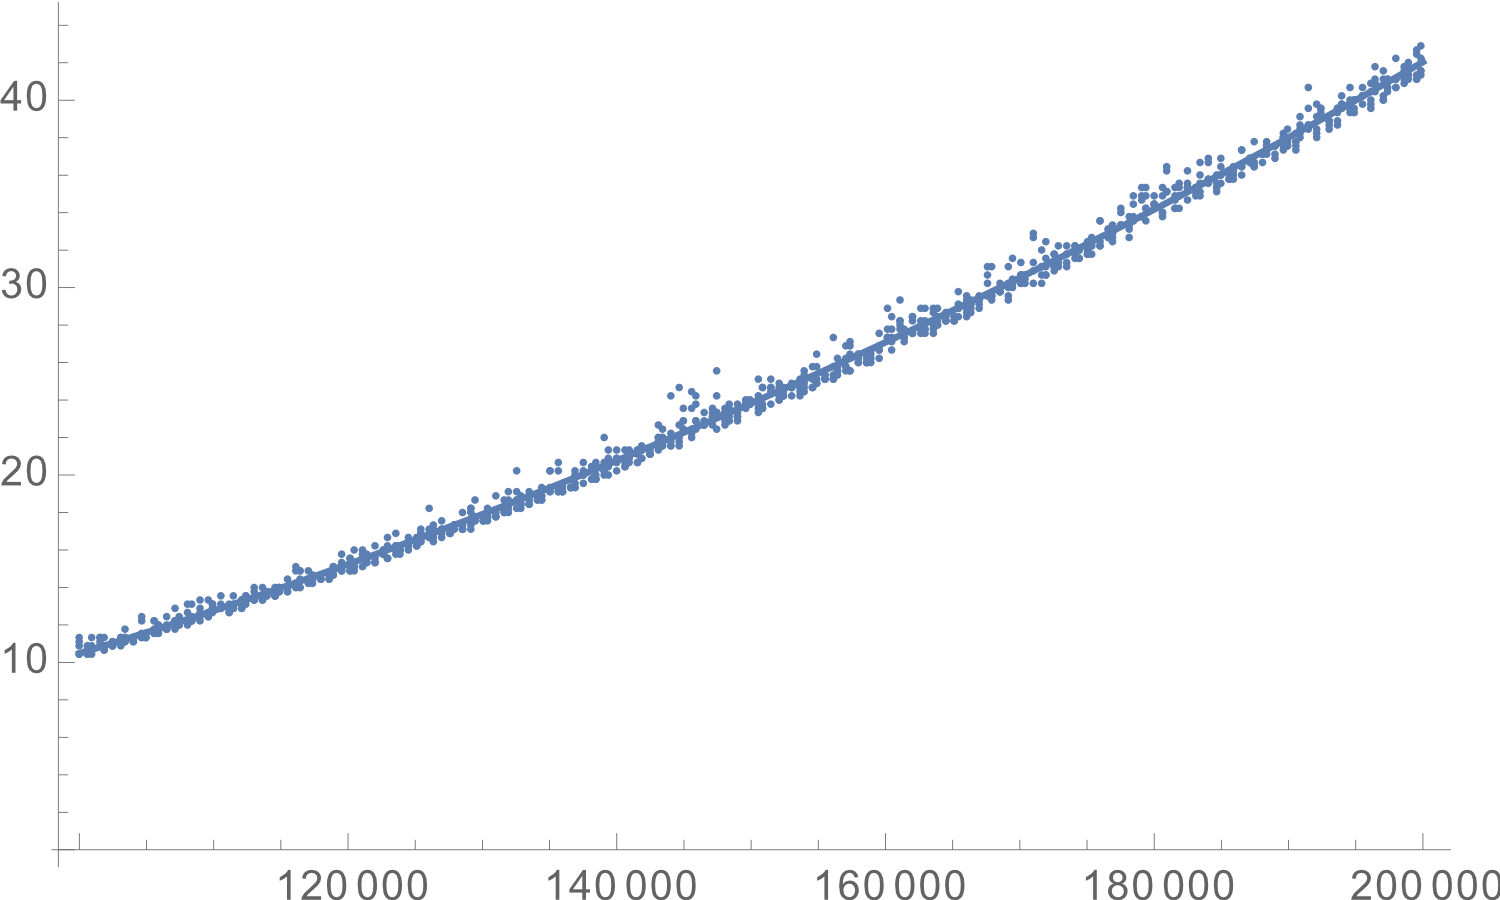
\includegraphics[width = \textwidth]{sortA_random_time.png}
        \caption{Time: \((9.7 \times 10^{-10}) n^2 + (2.4 \times 10^{-5}) n - 1.6\)}
    \end{subfigure}
    ~
    \begin{subfigure}[b]{0.45\textwidth}
        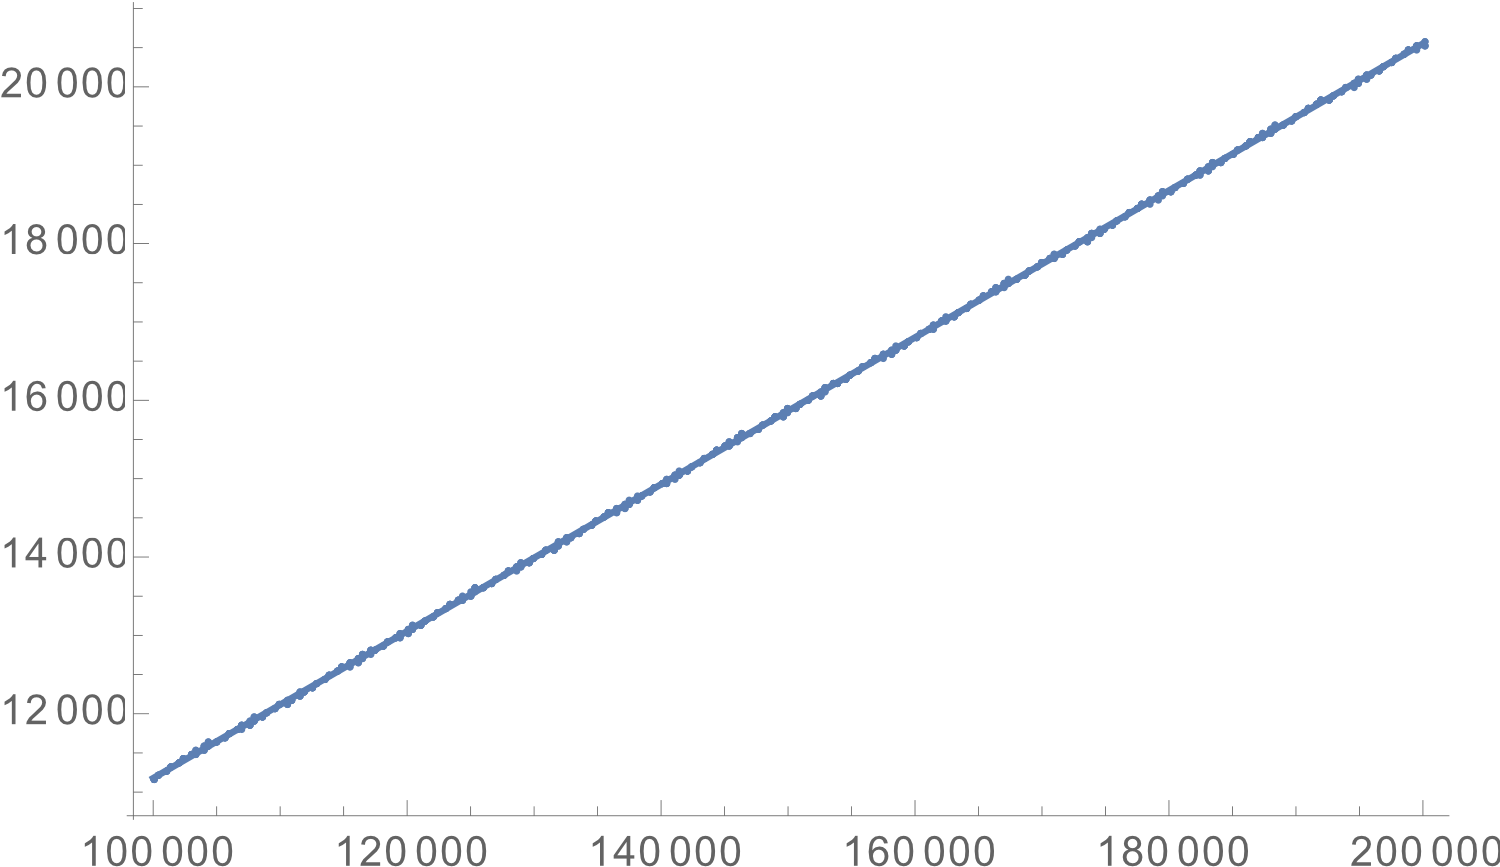
\includegraphics[width = \textwidth]{sortA_random_space.png}
        \caption{Space: \(0.094 n + 1800\)}
    \end{subfigure}
    \caption{Sort A - Random}
    \label{fig:sortA_random}
\end{figure}

\begin{figure}[p]
    \centering
    \begin{subfigure}[b]{0.45\textwidth}
        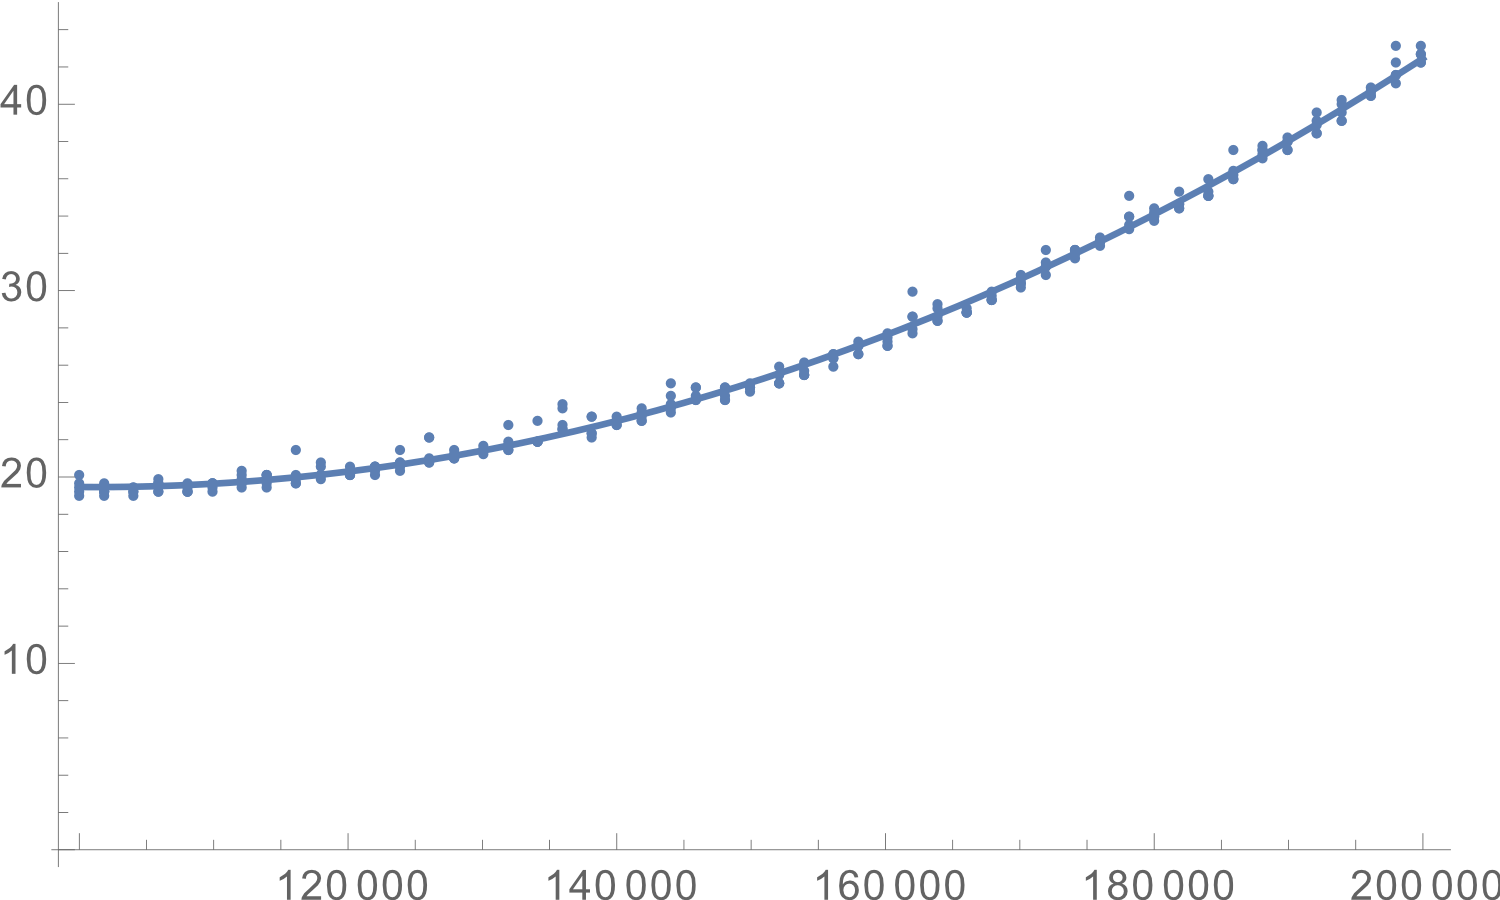
\includegraphics[width = \textwidth]{sortA_reverse_time.png}
        \caption{Time: \((2.4 \times 10^{-9}) n^2 - (4.8 \times 10^{-4}) n + 43\)}
    \end{subfigure}
    ~
    \begin{subfigure}[b]{0.45\textwidth}
        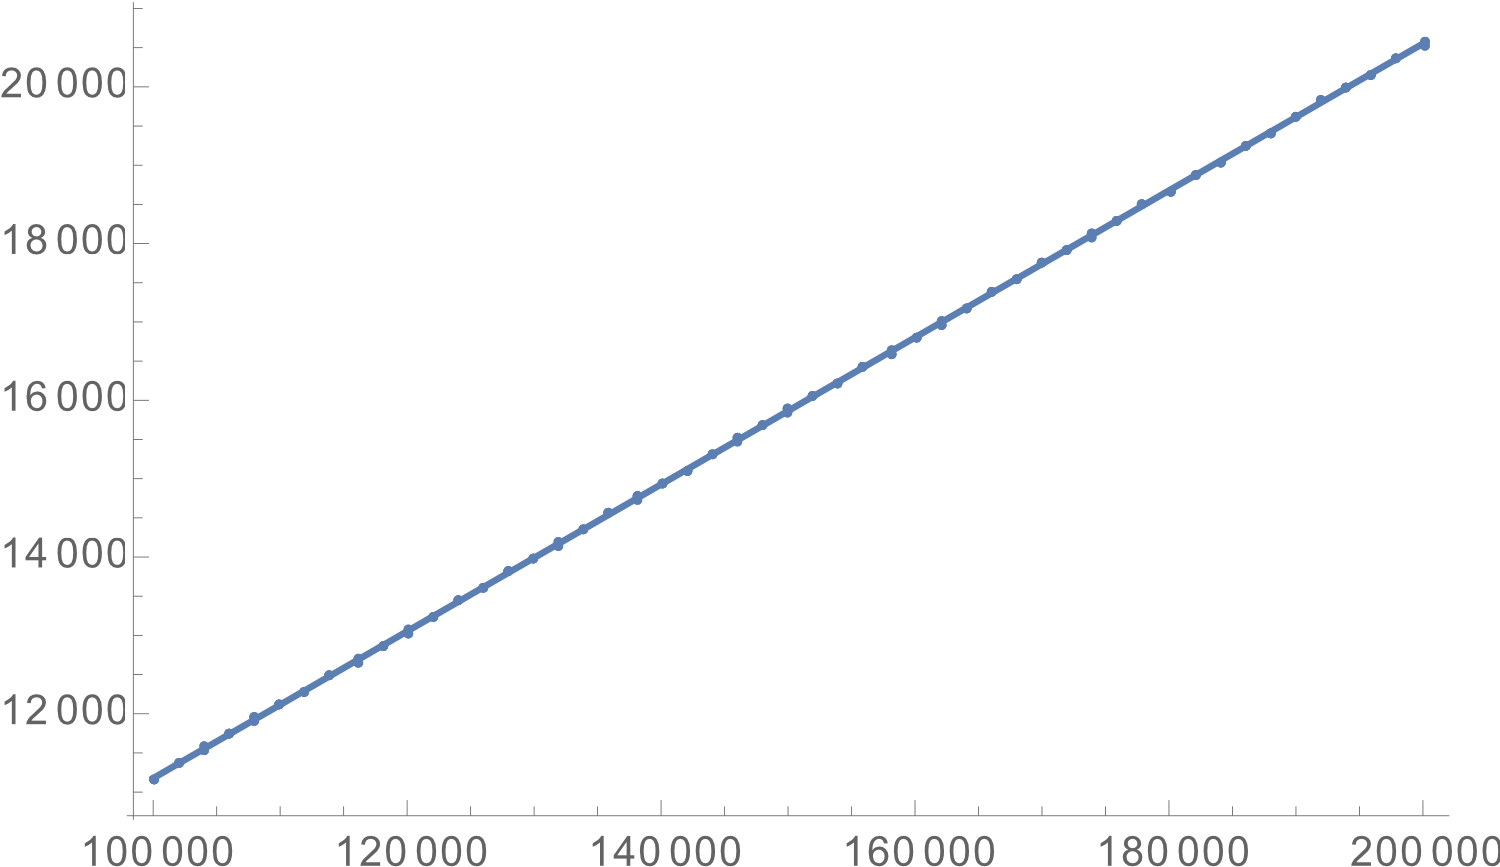
\includegraphics[width = \textwidth]{sortA_reverse_space.png}
        \caption{Space: \(0.094 n + 1800\)}
    \end{subfigure}
    \caption{Sort A - Reversed}
    \label{fig:sortA_reverse}
\end{figure}

\begin{figure}[p]
    \centering
    \begin{subfigure}[b]{0.45\textwidth}
        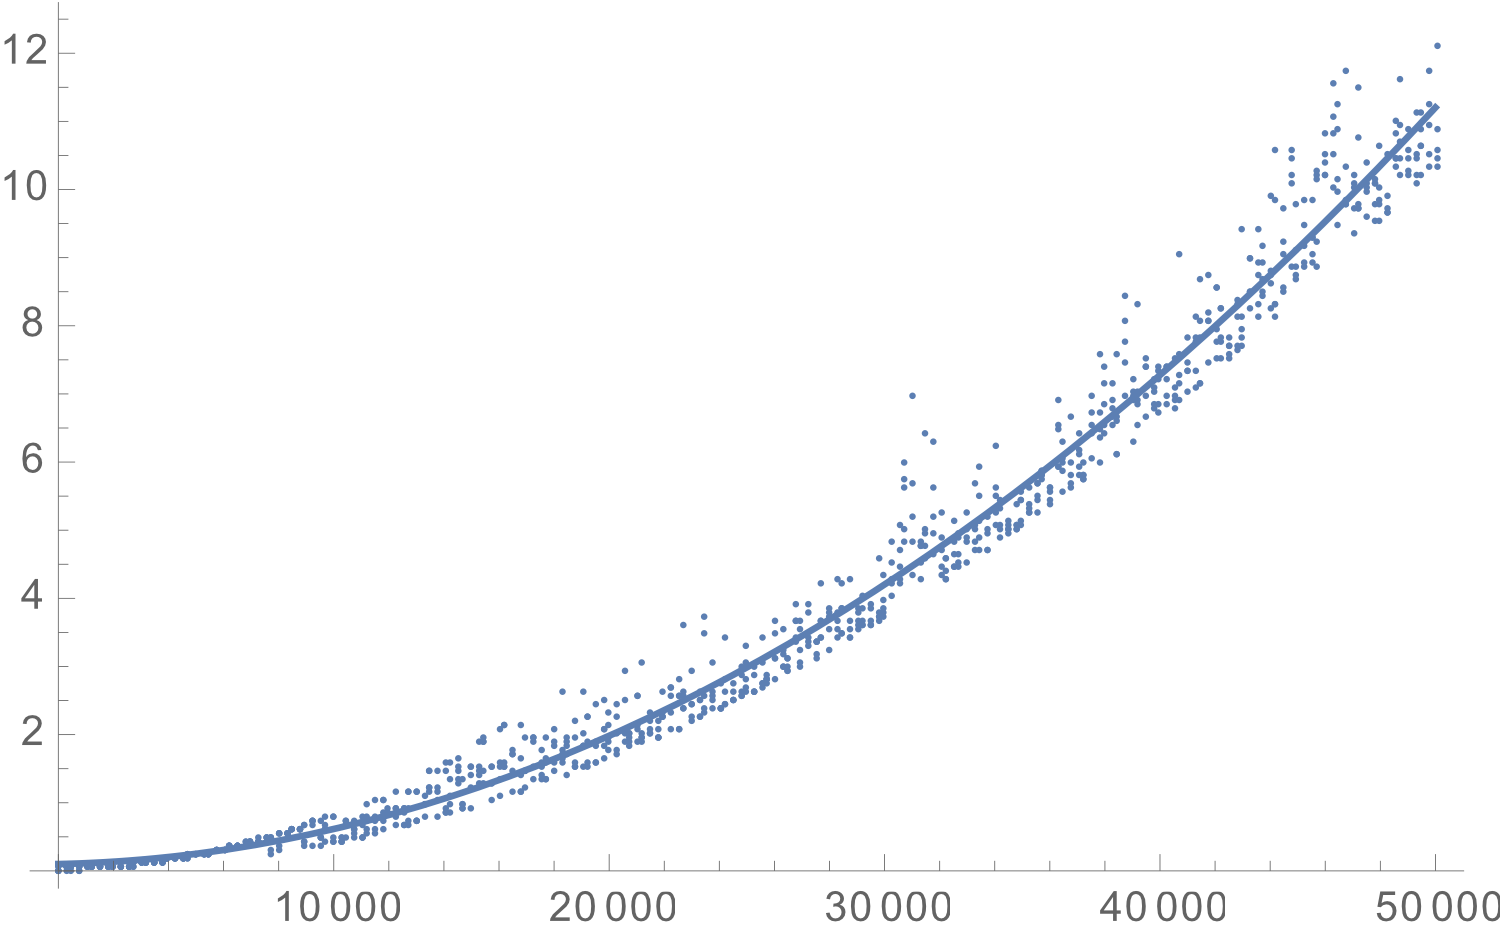
\includegraphics[width = \textwidth]{sortA_special_time.png}
        \caption{Time: \((4.3 \times 10^{-9}) k^2 + (8.8 \times 10^{-6}) k + 0.10\)}
    \end{subfigure}
    \caption{Sort A - Partly Ordered, Partly Reversed (\(n = 100000\))}
    \label{fig:sortA_special}
\end{figure}

\begin{figure}[p]
    \centering
    \begin{subfigure}[b]{0.45\textwidth}
        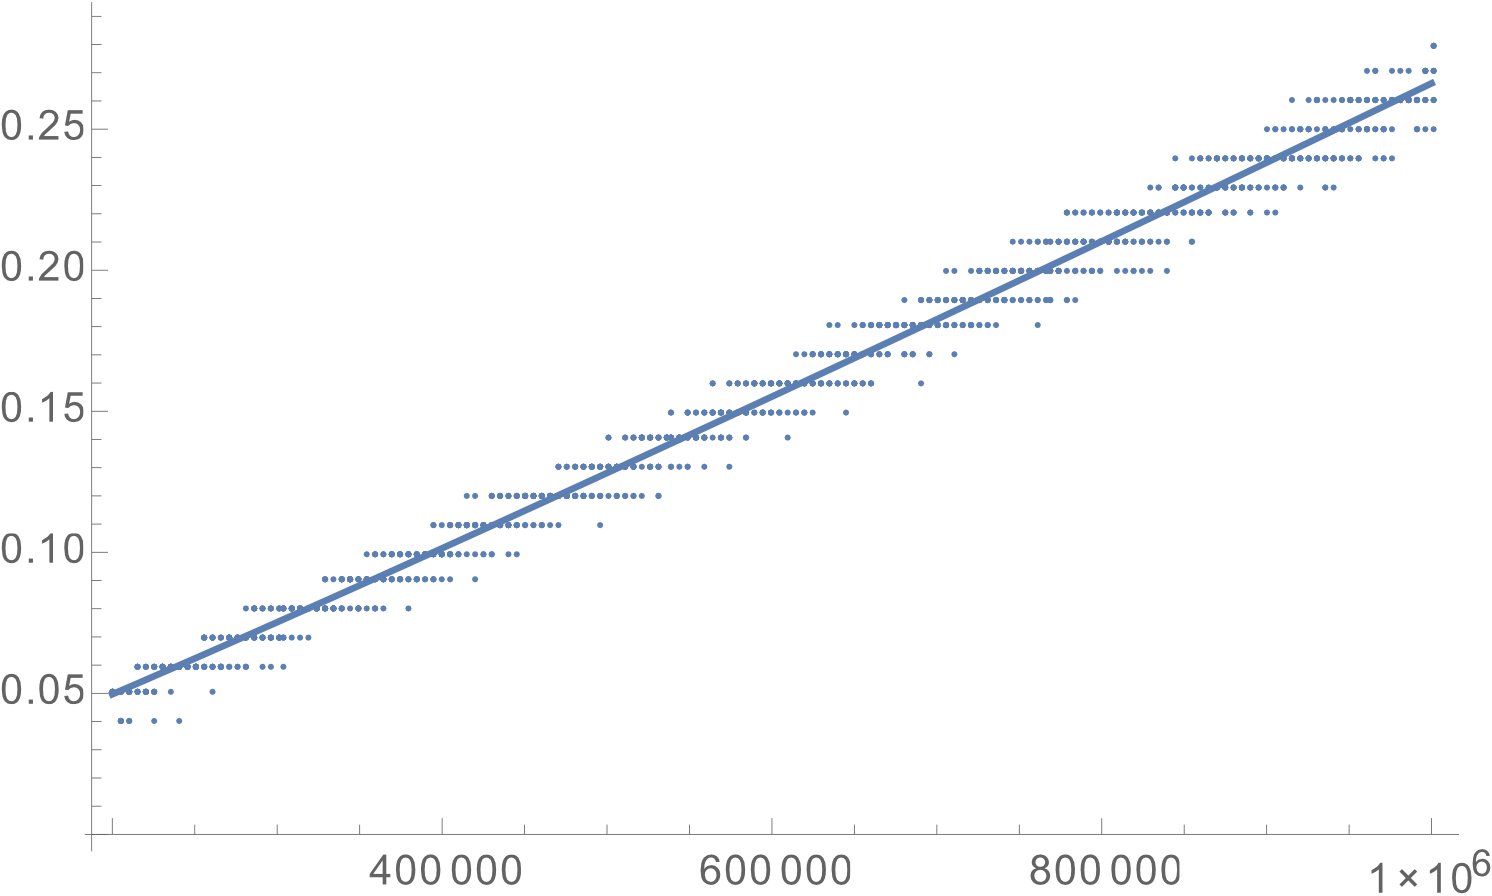
\includegraphics[width = \textwidth]{sortB_ordered_time.png}
        \caption{Time: \((1.9 \times 10^{-8}) n \ln{(n)} + 0.0032\)}
    \end{subfigure}
    ~
    \begin{subfigure}[b]{0.45\textwidth}
        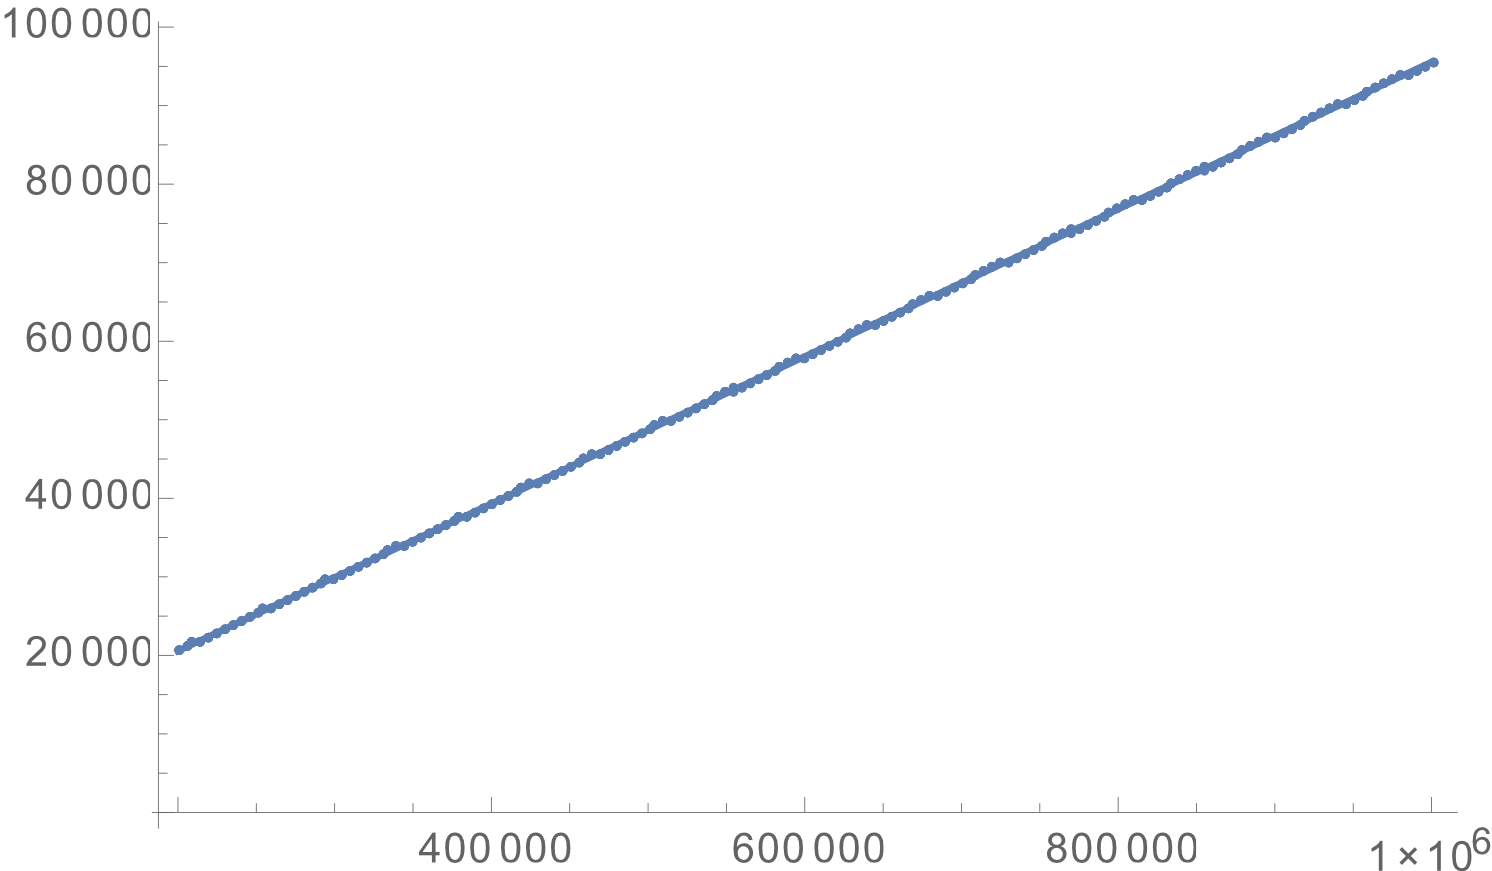
\includegraphics[width = \textwidth]{sortB_ordered_space.png}
        \caption{Space: \(0.094 n + 1800\)}
    \end{subfigure}
    \caption{Sort B - Ordered}
    \label{fig:sortB_ordered}
\end{figure}

\begin{figure}[p]
    \centering
    \begin{subfigure}[b]{0.45\textwidth}
        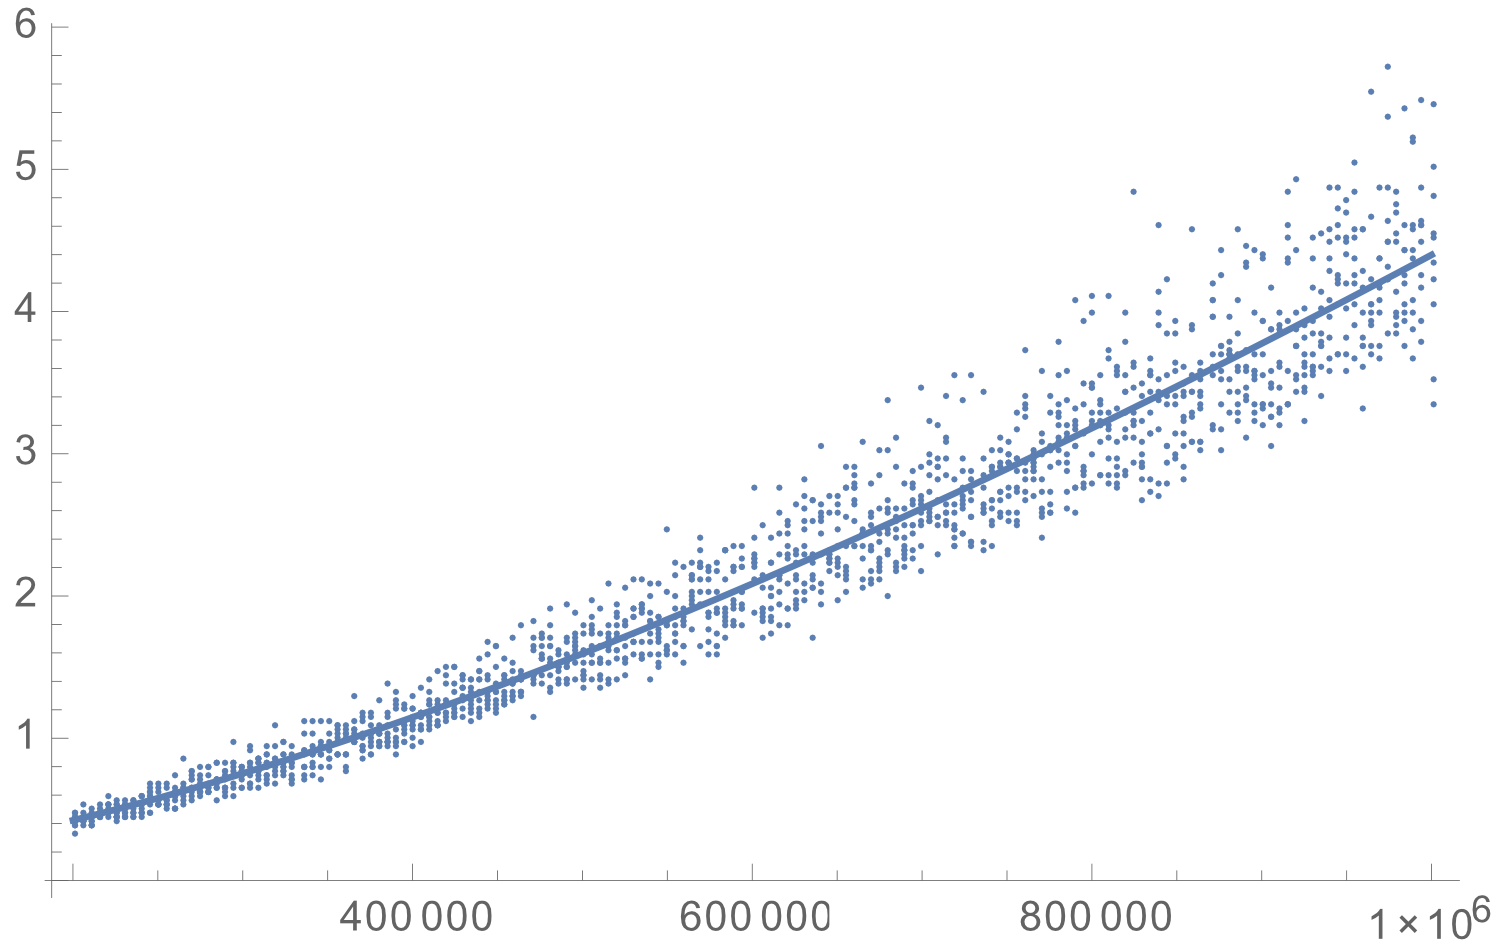
\includegraphics[width = \textwidth]{sortB_random_time.png}
        \caption{Time: \((2.6 \times 10^{-7}) n^\frac54 - (4.1 \times 10^{-6}) n + 0.12\)}
    \end{subfigure}
    ~
    \begin{subfigure}[b]{0.45\textwidth}
        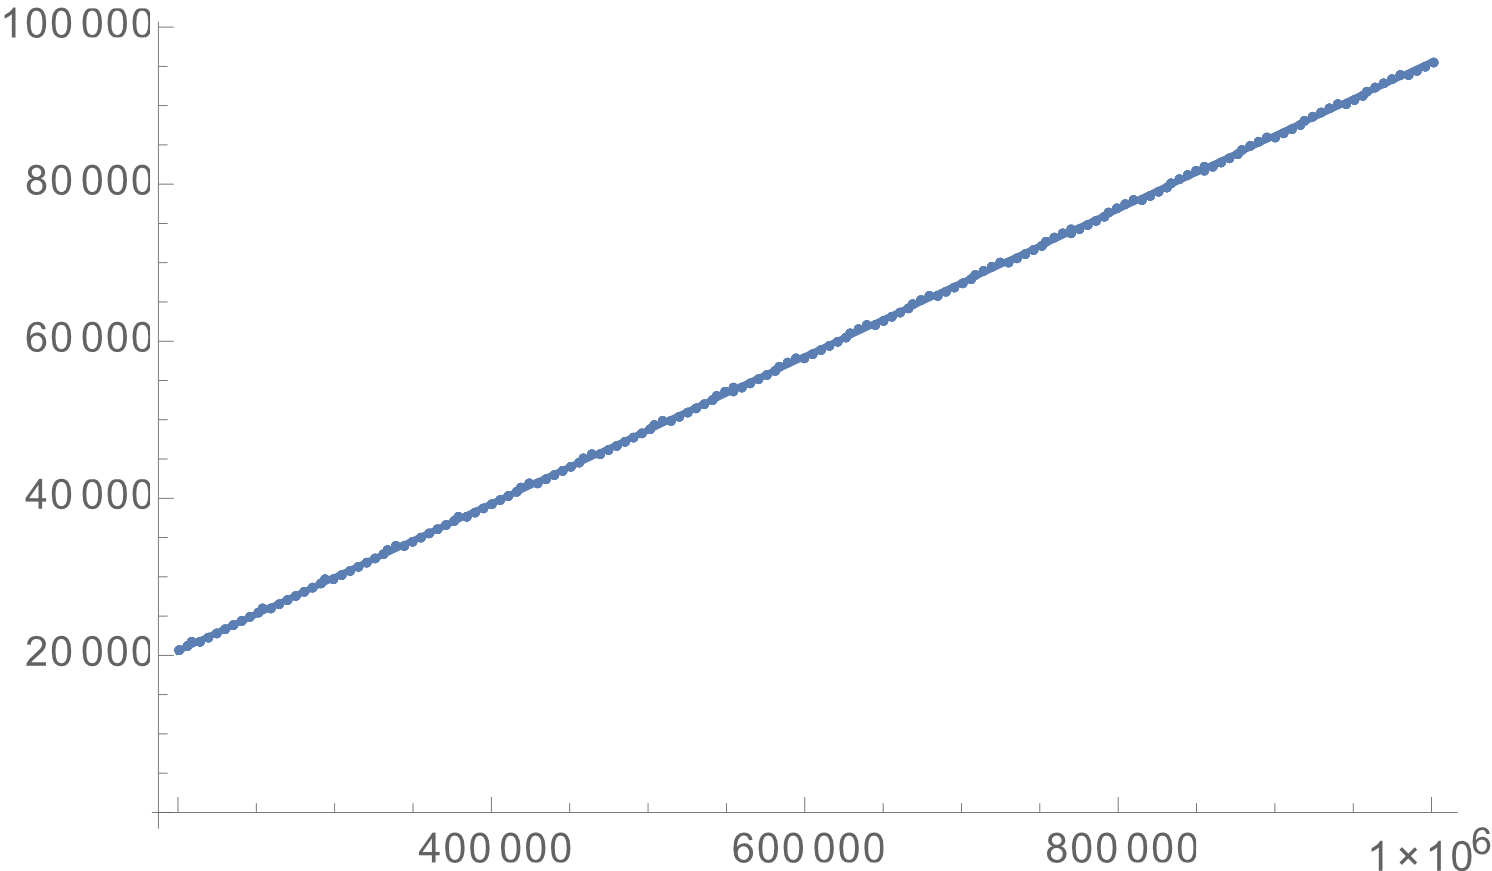
\includegraphics[width = \textwidth]{sortB_random_space.png}
        \caption{Space: \(0.094 n + 1800\)}
    \end{subfigure}
    \caption{Sort B - Random}
    \label{fig:sortB_random}
\end{figure}

\begin{figure}[p]
    \centering
    \begin{subfigure}[b]{0.45\textwidth}
        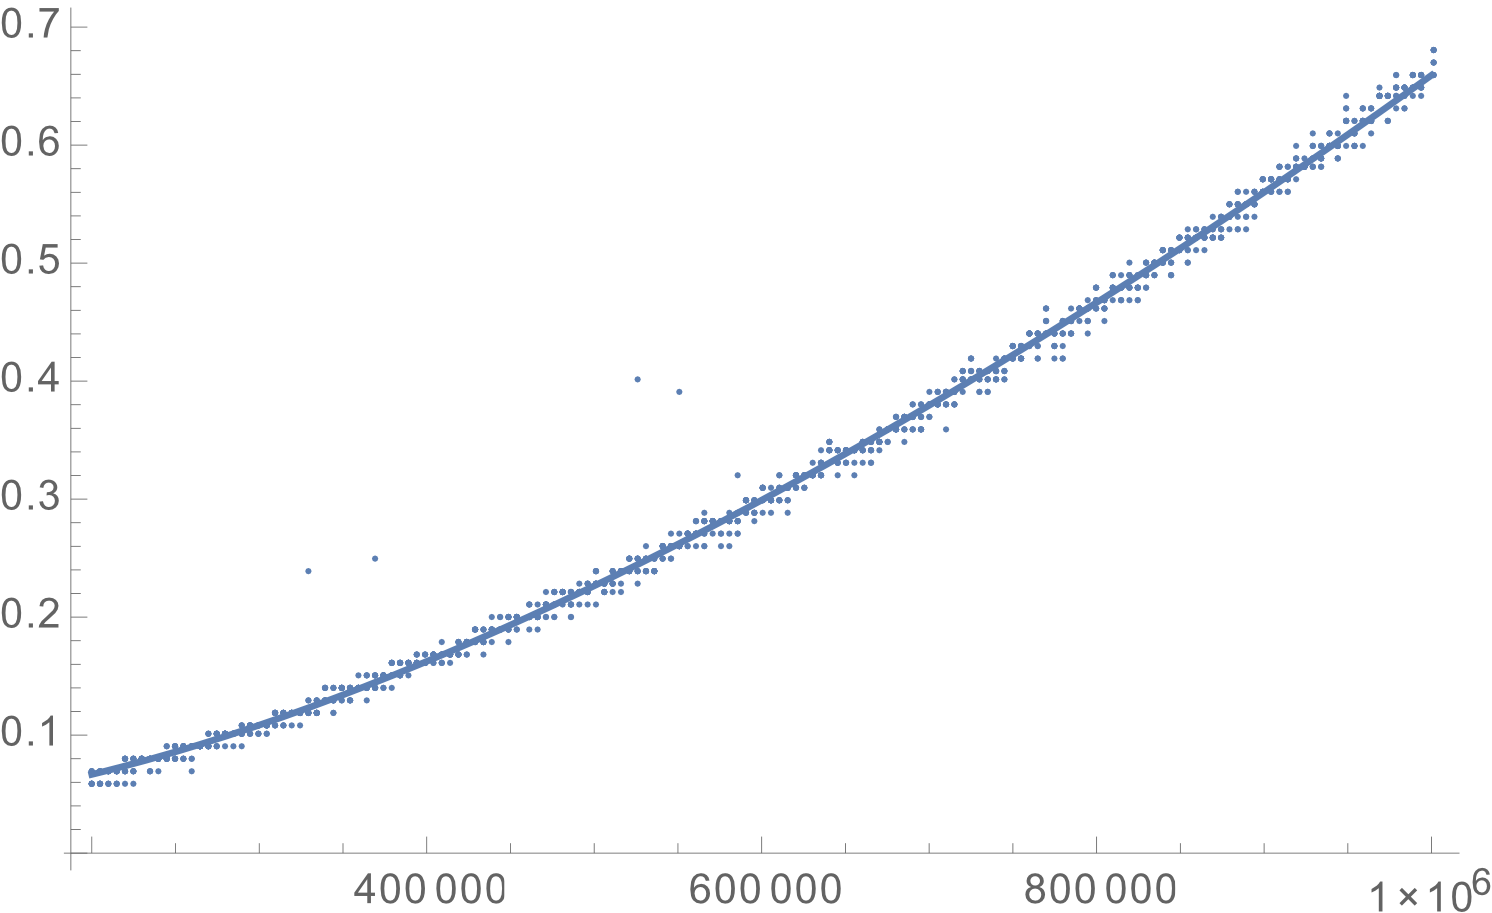
\includegraphics[width = \textwidth]{sortB_reverse_time.png}
        \caption{Time: \((1.2 \times 10^{-8}) n^\frac43 - (6.0 \times 10^{-7}) n + 0.045\)}
    \end{subfigure}
    ~
    \begin{subfigure}[b]{0.45\textwidth}
        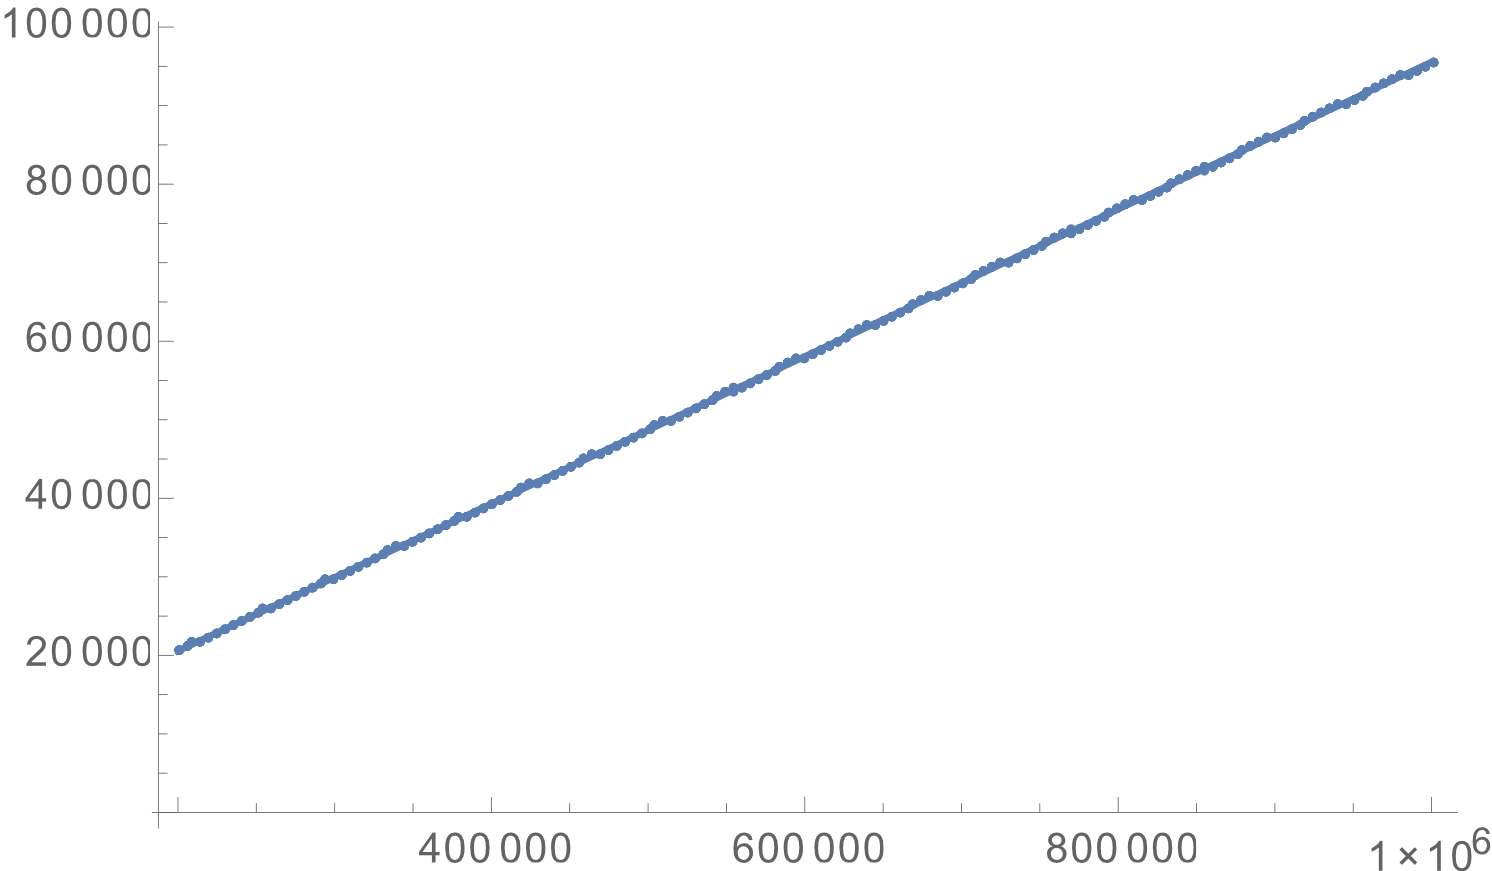
\includegraphics[width = \textwidth]{sortB_reverse_space.png}
        \caption{Space: \(0.094 n + 1800\)}
    \end{subfigure}
    \caption{Sort B - Reversed}
    \label{fig:sortB_reverse}
\end{figure}

\begin{figure}[p]
    \centering
    \begin{subfigure}[b]{0.45\textwidth}
        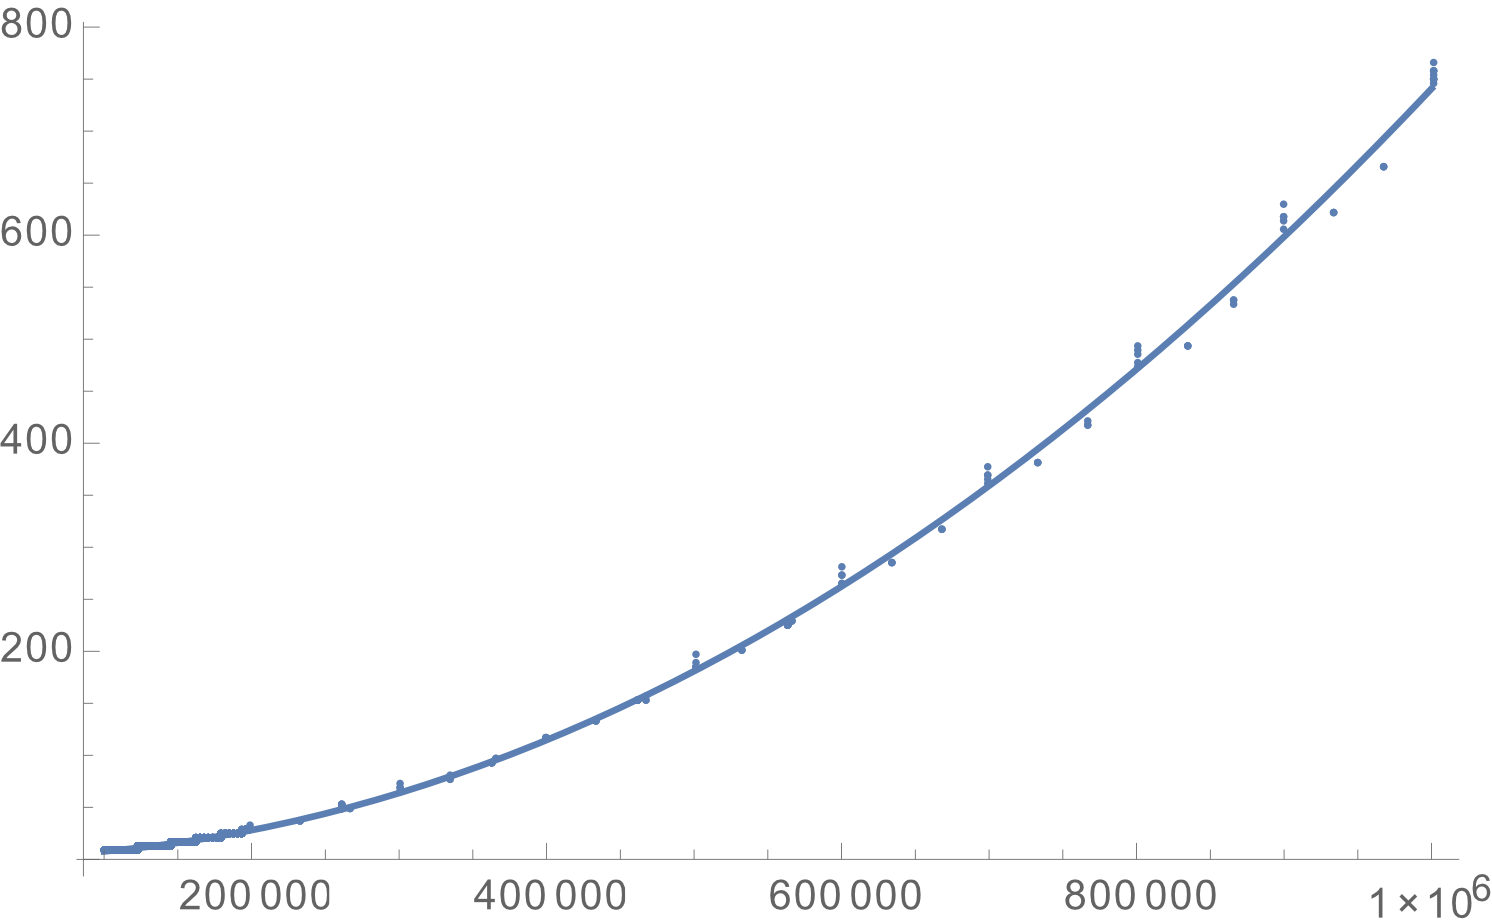
\includegraphics[width = \textwidth]{sortB_special_time.png}
        \caption{Time: \((7.6 \times 10^{-10}) n^2 - (1.9 \times 10^{-6}) n - 0.17\)}
    \end{subfigure}
    \caption{Sort B - Reversed, with all even index values higher than all odd index ones}
    \label{fig:sortB_special}
\end{figure}

\begin{table}
    \centering
    \begin{tabular}{c | c | c | c}
        Sort & Input Type & Time Complexity (s) & Space Complexity (kB) \\
        \hline
        & Ordered (Best) & \((5.7 \times 10^{-7}) n - 0.0019\) & \(0.094 n + 1800\) \\
        A & Random (Average/Worst) & \((9.7 \times 10^{-10}) n^2 + (2.4 \times 10^{-5}) n - 1.6\) & \(0.094 n + 1800\) \\
        & Reversed (Average/Worst) & \((2.4 \times 10^{-9}) n^2 - (4.8 \times 10^{-4}) n + 43\) & \(0.094 n + 1800\) \\
        & Special Case (\(n = 100000\)) & \((4.3 \times 10^{-9}) k^2 + (8.8 \times 10^{-6}) k + 0.10\) & \\
        \hline
        & Ordered (Best) & \((1.9 \times 10^{-8}) n \ln{(n)} + 0.0032\) & \(0.094 n + 1800\) \\
        B & Random (Average) & \((2.6 \times 10^{-7}) n^\frac54 - (4.1 \times 10^{-6}) n + 0.12\) & \(0.094 n + 1800\) \\
        & Reversed (Average) & \((1.2 \times 10^{-8}) n^\frac43 - (6.0 \times 10^{-7}) n + 0.045\) & \(0.094 n + 1800\) \\
        & Special Case (Worst) & \((7.6 \times 10^{-10}) n^2 - (1.9 \times 10^{-6}) n - 0.17\) &
    \end{tabular}
    \caption{Raw fitted functions}
    \label{tab:raw_fit}
\end{table}

From the fitted functions of the results (Table \ref{tab:raw_fit}), Sort A has \(O(n)\) best case while there was no real distinguishment between average and worst case, both being \(O(n^2)\). Additionally. when testing the special case, Sort A displayed \(O(k^2)\) time complexity where \(k\) was the number of unsorted elements. It was also measured to be stable.

Meanwhile, Sort B demonstrated a variation of complexities, with a best case \(O(n \log(n)\) and worst and average case of \(O(n^\frac43)\) and \(O(n^\frac54)\) respectively. When attempting to distinguish between Shell and Quick sorts with a riffle sorted list, Sort B displayed \(O(n^2)\) complexity. It was also measured to be unstable, but the same input data produced the same output, so was also pure.

\section{Discussion}
Sort A can be concluded to be Insertion Sort with Table \ref{tab:complexity}. Through a comparison of Best/Worst/Average cases Sort A could be narrowed down to either Insertion or Early Eixt Bubble Sort. However, testing with a partially ordered and reversed data set allowed us to conclude, since Sort A did not exhibit \(O(n k)\) complexity, it was conclusively Insertion Sort. Sort B is highly likely to be \(4^n\) Shell Sort, with the special case \(O(n^2)\) complexity, distinguishing it from Quicksort and Sedgewick Shell Sort, and the unstable but pure output.

\end{document}